\chapter{Исследовательская часть}

%\section{Пример работы}

%Демонстрация работы программы приведена на рисунке \ref{img:levenshtein_demo}.

%\boximg{160mm}{levenshtein_demo}{Демонстрация работы алгоритмов нахождения расстояния Левенштейна и Дамерау -- Левенштейна}

\section{Технические характеристики}

Технические характеристики устройства, на котором выполнялось тестирование:

\begin{itemize}
	\item Операционная система: Windows 10.
	\item Память: 16 GiB.
	\item Процессор: Intel(R) Core(TM) i7-4700HQ CPU @ 2.40GHz.
\end{itemize}


\section{Временные характеристики}

Для сравнения времени выполнения программ брались строки длиной [10, 20, 30, 50, 100, 200] символов. Для получения точных временных характеристик замеры времени прогонялись 500 раз. 

\begin{figure}[h]
    \centering
    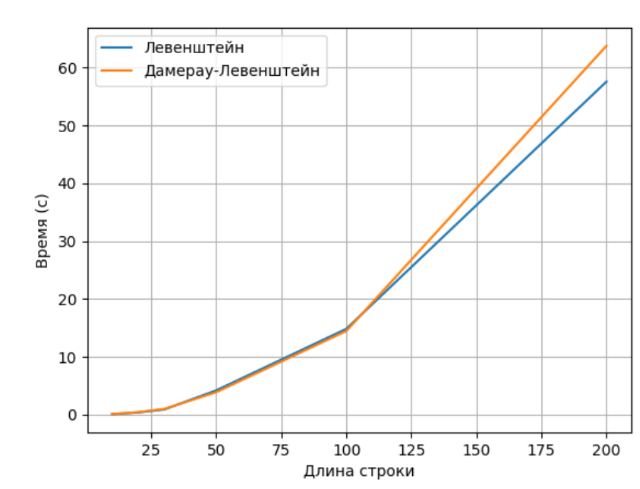
\includegraphics[width=130mm]{inc/img/timing.png}
    \caption{Сравнение времени работы алгоритма поиска расстояния Левенштейна и Дамерау-Левенштейна}
    \label{img:timing}
\end{figure}


   
Из рисунка \ref{img:timing} видно, что при короткой длине разница по времени минимальна, при увеличении длины алгоритм поиска расстояния Левенштейна с небольшим опережением вырывается вперед.




\section{Характеристики по памяти}

Алгоритмы нахождения расстояний Левенштейна и Дамерау — Левенштейна не отличаются друг от друга с точки зрения использования памяти, следовательно, достаточно рассмотреть лишь разницу рекурсивной и матричной реализаций этих алгоритмов.

Максимальная глубина стека вызовов при рекурсивной реализации равна сумме длин входящих строк, при этом для каждого вызова рекурсии в моей реализации требуется:
\begin{itemize}
    \item перeменная типа int, в моем случае: $4 $ байта;
    \item 2 аргумента типа строка: $2 \cdot 24 = 48$ байт;
    \item адрес возврата: 8 байт;
    \item место для записи возвращаемого функцией значения: 8 байт.
\end{itemize}
Таким образом получается, что при обычной рекурсии на один вызов требуется (\ref{for:onecall}): 

\begin{equation}
M_{per call} = 4 + 48 + 8 + 8 = 68 байт
\label{for:onecall}
\end{equation}

Следовательно память, расходуемая в момент, когда стек вызовов максимален, равна (\ref{for:rec}): 

\begin{equation}
    M_{recursive} = 80 \cdot depth
\label{for:rec}
\end{equation}

где \textit{depth} - максимальная глубина стека вызовов, которая равна (\ref{for:depth}):

\begin{equation}
depth = |S_1| + |S_2|
\label{for:depth}
\end{equation}

где $S_1, S_2$ - строки.


Память, требуемая для при итеративной реализации, состоит из следующего:
\begin{itemize}
    \item 2 локальные перeменные типа int, в моем случае: $2 \cdot 4 = 8$ байт;
    \item 2 аргумента типа строка: $2 \cdot 24 = 48$ байт;
    \item адрес возврата: 8 байт;
    \item место для записи возвращаемого функцией значения: 8 байт;
    \item матрица: $M_{Matrix}$ размером $4 \cdot (n + 1) \cdot (m + 1)$.
\end{itemize}

Таким образом общая расходуемая память итеративных алгоритмов (\ref{for:iter}):

\begin{equation}
M_{iter} = M_{Matrix} + 72
\label{for:iter}
\end{equation}


\section*{Вывод}

В данном разделе было произведено сравнение количества затраченного времени и памяти вышеизложенных алгоритмов. Самым быстрым оказался матричный алгоритм нахождения расстояния Левенштейна.